\subsubsection{Partially Mapped Crossover (PMX)}
\label{sec:keen:op:cx:partially_mapped}
  Partially Mapped Crossover (PMX) is another robust permutation crossover 
  technique highly regarded in the world of genetic algorithms. Introduced by 
  Goldberg and Lingle~\autocite{goldbergAllelesLociTraveling1985}, it primarily 
  caters to problems that involve ordering or sequencing, much like the TSP. PMX 
  has been conceived to ensure output inherit a blend of both input 
  chromosomes without disturbing the position-based information vital for many 
  sequencing problems.

  \begin{definition}[Partially Mapped Crossover]
    The \textit{partially mapped crossover} (PMX) operates by choosing a random 
    substring of one input chromosome and then mapping the position of these 
    genes on the other input chromosome. This procedure ensures output 
    obtain genes from both inputs, maintaining the original order. Formally, 
    PMX can be articulated as:

    \begin{equation}
      X_\mathrm{pmx} :\: 
        \mathbb{P} \times [0,\, 1] \times [0,\, 1] \times \{0,\, 1\} \rightarrow \mathbb{P};\;
        (P,\, \rho_\mathbf{i},\, \rho_\mathbf{c}, e) \mapsto X_\mathrm{pmx}(P,\, \rho_\mathbf{i},\, \rho_\mathbf{c}, e)
    \end{equation}

    where:

    \begin{itemize}
      \item \(P\) denotes a population of sequenced chromosomes.
      \item \(\rho_\mathbf{i}\) stands for the likelihood of the crossover being applied to an individual.
      \item \(\rho_\mathbf{c}\) signifies the probability of triggering the PMX operation on a chromosome.
      \item \(e\) is a boolean value that determines whether the same individual can be used more than once as a parent.
    \end{itemize}
  \end{definition}

  The implementation of PMX in the \textit{Keen} framework operates as follows:

  \begin{code}{
      PMX algorithm as described in the \textit{Keen} framework.
  }{
      label={lst:keen:op:cx:pmx}
  }{kotlin}
    (output1, output2) = input1, input2
    (lo, hi) = random.indices in input1
    crossSection1 = input1[lo..hi]
    crossSection2 = input2[lo..hi]
    for (i in 0..input1.size) {
        if (i < lo or i >= hi) {
            while (output1[i] in crossSection2) {
                index = crossSection2.indexOf(output1[i])
                output1[i] = crossSection1[index]
            }
            while (output2[i] in crossSection1) {
                index = crossSection1.indexOf(output2[i])
                output2[i] = crossSection2[index]
            }
        }
    }
    return output1, output2
  \end{code}

  The essence of the above implementation is to select a random section from the
  first input chromosome and copy it to the output chromosome in the same
  position. Then, the genes from the second input chromosome, not in the copied
  section, fill the output in the same position as the first input. Finally,
  the remaining genes are mapped from the second input chromosome to the
  output chromosome, ensuring that the output chromosome is a valid
  permutation. 
  
  Consider the following example:
  \paragraph{Initial Chromosomes}

    Let's begin with two input chromosomes:

    \begin{itemize}
      \item \(\mathbf{I}_1 = 1\,2345\,6789\)
      \item \(\mathbf{I}_2 = 5\,7491\,3628\).
    \end{itemize}

  \paragraph{Section Selection}

    Next, a random section from the first input chromosome is selected. For 
    instance, consider the section \(\textbf{I}_1[3\dots6] = 3456\). This 
    section is replaced with the equivalent section from the second input 
    chromosome, \(\textbf{I}_2[3\dots6] = 4913\). The resulting intermediate 
    output looks like \(\_\,\_\,4913\_\,\_\,\_\).

  \paragraph{Gene Transfer}

    The next step involves copying genes. Any genes from the first input 
    chromosome not present in the copied section are transferred to the output 
    chromosome, keeping their original positions. This action results in the 
    intermediate output: \(\_\,2\,4913\,7\_\).

  \paragraph{Gene Mapping}
    The final step is gene mapping. Here, remaining genes from the second input 
    chromosome are mapped onto the output chromosome. The aim is to form a valid 
    permutation. Genes already present in the output chromosome get replaced by 
    corresponding genes from the second input chromosome. This process might 
    require repeated iterations if the mapped gene is already in the output 
    chromosome. The mapping is continued until all genes find their places. 

    To clarify with an example:

    \begin{enumerate}
      \item Start with the gene \enquote{1} from the first position of 
        \(\mathbf{I}_1\). 
        Locate its position in the output and replace it with gene \enquote{5} 
        from \(\mathbf{I}_2\), producing the intermediate sequence 
        \(5\,249137\,\_\).
      \item Take gene \enquote{9} from the last position of \(\mathbf{I}_1\). 
        Finding its position in the output reveals another \enquote{9}. Thus, 
        refer back to \(\mathbf{I}_1\) and take the gene \enquote{4}. Since it 
        maps to \enquote{3}, which is already in the output, turn to gene 
        \enquote{3} in \(\mathbf{I}_1\). This maps to \enquote{6} from 
        \(\mathbf{I}_2\), which is finally placed in the output, resulting in 
        \(\textbf{O}_1 = 5249137\,6\).
    \end{enumerate}

  \paragraph{Visualization}
    For a clearer visual representation of this entire process, refer to \vref{fig:keen:op:cx:pmx}.

    \begin{figure}[ht!]
      \centering
      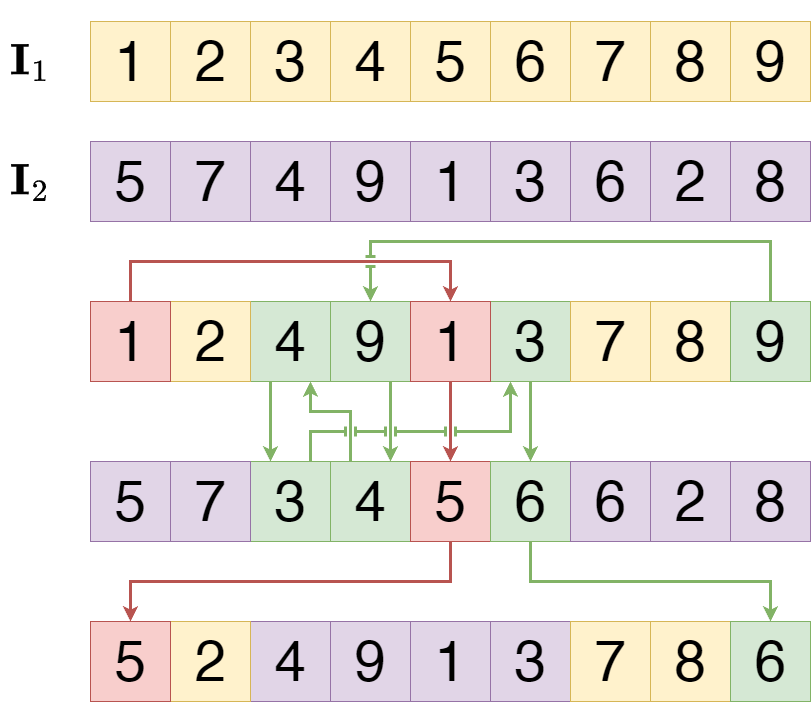
\includegraphics[width=0.5\textwidth]{img/keen/PMX.png}
      \caption{Partially Mapped Crossover (PMX) operator.}
      \label{fig:keen:op:cx:pmx}
    \end{figure}
